\documentclass{article}
\usepackage{enumerate}
\usepackage{amsmath}
\usepackage{amssymb}
\usepackage{graphicx}
\usepackage{subfigure}
\usepackage{geometry}
\usepackage{caption}
\usepackage{indentfirst}
\usepackage[colorlinks,urlcolor=blue]{hyperref}
\usepackage{minted}
\usemintedstyle{autumn}
\setminted{linenos,breaklines,tabsize=4,xleftmargin=1.5em}
\geometry{left=3.0cm,right=3.0cm,top=3.0cm,bottom=4.0cm}
\title{VE370 Project 1}
\author{Liu Yihao 515370910207}
\date{}

\begin{document}
\maketitle

\section{Objectives}
Develop a MIPS assembly program that operates on a data segment consisting of an array of 32-bit unsigned integers. In the text (program) segment of memory, write a procedure called main that implements the main() function and other subroutines described below. Assemble, simulate, and carefully comment the file. Screen print your simulation results and explain the results by annotating the screen prints. You should compose an array whose size is determined by you in the main function and is not less than 20 elements. 

\begin{minted}{c}
main() {
    int size = ...;  //determine the size of the array here
    int PassCnt, FailCnt;							
    int testArray[size] = { 55, 83,   
        ... //compose your own array here
    };				
    PassCnt = countArray(testArray, size, 1);						
    FailCnt = countArray(testArray, size, -1);						
}		
								
int countArray(int A[], int numElements, int cntType) {					
/**********************************************************************
* Count specific elements in the integer array A[] whose size is     *
* numElements and return the following:                              *
*                                                                    *
* When cntType = 1, count the elements greater than or equal to 60;  *
* When cntType = -1, count the elements less than 60;                *
**********************************************************************/
    int i, cnt = 0;									
    for(i = numElements - 1; i > -1; i--) {						
	    switch (cntType) {								
            case '1' : cnt += Pass(A[i]); break;			
            otherwise: cnt += Fail(A[i]); 			
	    }								
    }							
    return cnt;							
}							
							
int Pass(int x) {							
    if(x >= 60) return 1;						
    else return 0;						
}							
							
int Fail(int x) {							
    if (x < 60) return 1;						
    else return 0;						
}
\end{minted}

\section{Procedure}
The effects of all MIPS statements are carefully commented, so I won't show many details here.

\subsection{main function}
In the main function, I use the stack to save the scores. I choose 50 as the size, and I write a python script to generate the data, uniformly distributed in $[0,100]$.
\inputminted{python}{testArray.py}

Then I called the function countArray for two times to count the pass and fail number. I also use the stack the save ascii strings ``Pass: '', ``Fail: '' and ``\textbackslash n'' so that you can see a user friendly result on the console.

\subsection{countArray function}
In the countArray function, I use saved registers \$s0, \$s1, \$s2, \$s3, \$s4, and I call other functions, so these registers and \$ra should be saved into stack in the begin and load from the stack in the end. Then I write a for loop and a condition statement, so some jump tags is added.

\subsection{Pass and Fail function}
Theses two function are very easy, no stack space is needed, only a condition statement can give the correct result.

\section{Result}
I use the data [55, 83, 21, 20, 40, 49, 42, 35, 92, 8, 65, 88, 25, 100, 43, 9, 98, 10, 81, 63, 83, 27, 42, 81, 94, 2, 40, 49, 75, 46, 67, 46, 89, 27, 39, 12, 19, 41, 86, 3, 14, 64, 22, 64, 8, 38, 32, 26, 64, 5], there are 50 in total, 18 pass, 22 fail. \\

The simulation result is shown in Figure \ref{fig-console}.

\begin{figure}[!htbp]
\centering
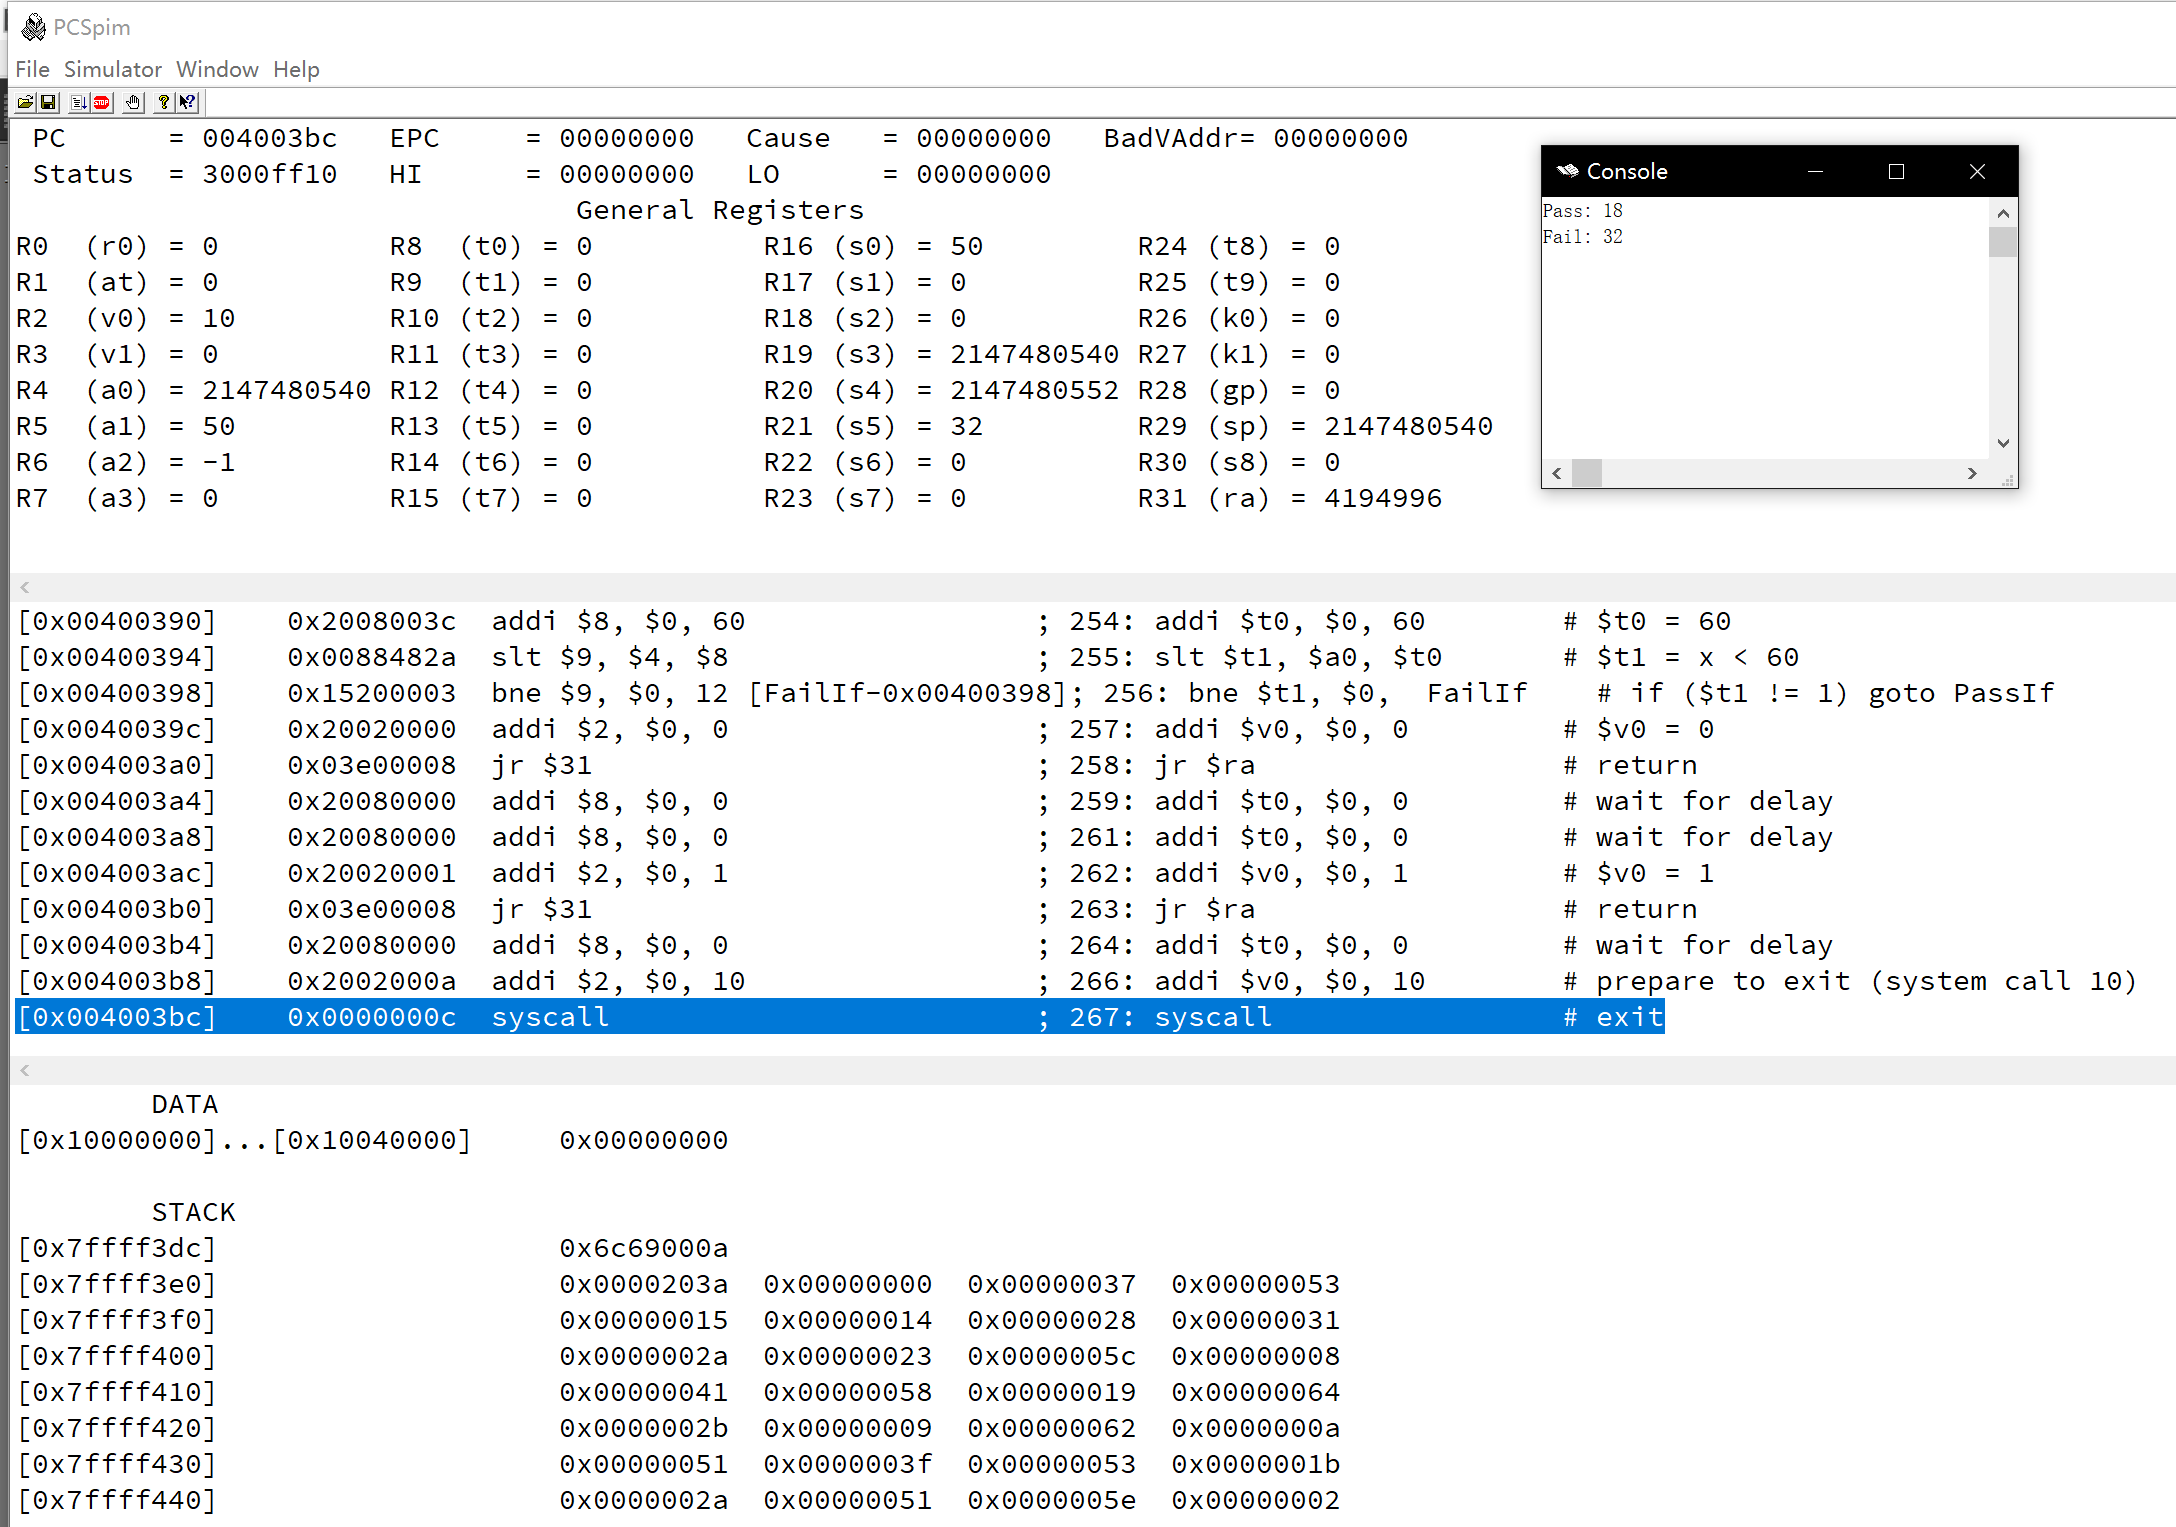
\includegraphics[width=\linewidth]{console.png}
\caption{Simulation result}
\label{fig-console}
\end{figure}

\section{Conclusion}
The things I want to mention are mainly in two aspects.\\

First, programming in pseudo instructions is much more efficient then without them. I made a mistake that I didn't switch off this option, and I found many pseudo instructions on the Internet. I used the .data scope to save ascii and word, with the usage of la instruction. However, pseudo instructions are not permitted, so I have to change them into silly assignment on stack (I know a c compiler will put these static data on the global variable area).\\

Second, the delay in branches and loads is quite confusing. I added many no-effect statement after jr, jal and lw to avoid the skip of those useful statements. I wondered whether the delay should be considered in a real assembly environment.

\section{Appendix}
\inputminted{asm}{p1.s}



\end{document}
